\documentclass[aspectratio=169]{beamer}

% Theme
\usetheme{Madrid}
\usecolortheme{whale}

% Packages
\usepackage[utf8]{inputenc}
\usepackage{tikz}
\usepackage{listings}
\usepackage{booktabs}

% TikZ libraries
\usetikzlibrary{shapes, arrows, positioning}

% Colors
\definecolor{primaryblue}{RGB}{0, 102, 204}
\definecolor{successgreen}{RGB}{40, 167, 69}
\definecolor{dangerred}{RGB}{220, 53, 69}

% Title
\title[Introduction]{Introduction to Software Development Projects}
\subtitle{CS2113 -- Software Development Project}
\author{Masoud Hamad}
\institute{School of Computing Communication and Media Studies}
\date{Academic Year 2025}

\begin{document}

%============================================================
\begin{frame}
    \titlepage
\end{frame}

%============================================================
\begin{frame}{Outline}
    \tableofcontents
\end{frame}

%============================================================
\section{What is a Software Development Project?}
%============================================================

\begin{frame}{What is a Software Development Project?}
    \begin{itemize}
        \item Software projects emerge when there's \textbf{identified need} and \textbf{funding}
        \item Projects vary from months to years
        \item Involve \textbf{stakeholders} -- all people affected by the software
        \begin{itemize}
            \item End users
            \item Funding customers
            \item Development team
        \end{itemize}
    \end{itemize}

    \vspace{0.5cm}

    \begin{alertblock}{Key Insight}
        Most development problems are \textbf{non-technical} rather than technical!
    \end{alertblock}
\end{frame}

%============================================================
\begin{frame}{Development Team Structure}
    \begin{center}
    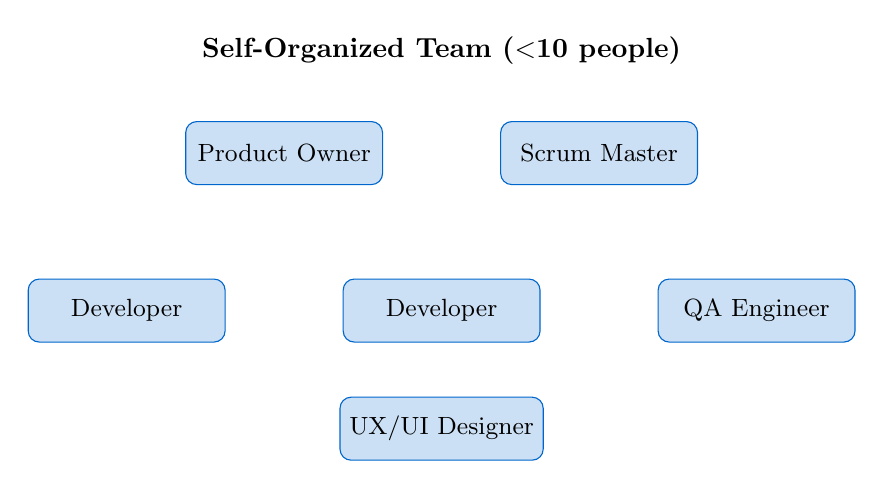
\begin{tikzpicture}[
        role/.style={rectangle, draw=primaryblue, fill=primaryblue!20, rounded corners, minimum width=2.5cm, minimum height=0.8cm, align=center, font=\small}
    ]
        \node[role] (po) at (0, 2) {Product Owner};
        \node[role] (sm) at (4, 2) {Scrum Master};
        \node[role] (dev1) at (-2, 0) {Developer};
        \node[role] (dev2) at (2, 0) {Developer};
        \node[role] (qa) at (6, 0) {QA Engineer};
        \node[role] (ux) at (2, -1.5) {UX/UI Designer};

        \node[font=\bfseries, above] at (2, 3) {Self-Organized Team ($<$10 people)};
    \end{tikzpicture}
    \end{center}
\end{frame}

%============================================================
\section{Agile Principles}
%============================================================

\begin{frame}{The Agile Manifesto}
    \begin{block}{We value:}
        \begin{enumerate}
            \item \textbf{Individuals and interactions} over processes and tools
            \item \textbf{Working software} over comprehensive documentation
            \item \textbf{Customer collaboration} over contract negotiation
            \item \textbf{Responding to change} over following a plan
        \end{enumerate}
    \end{block}

    \vspace{0.5cm}

    \begin{exampleblock}{Critical Value}
        Welcome change -- requirements frequently shift during development!
    \end{exampleblock}
\end{frame}

%============================================================
\section{Software Development Lifecycle}
%============================================================

\begin{frame}{SDLC Phases}
    \begin{columns}
        \begin{column}{0.5\textwidth}
            \begin{enumerate}
                \item \textbf{Requirements} -- Collect stakeholder needs
                \item \textbf{Design} -- Analyze and identify solutions
                \item \textbf{Implementation} -- Write code
                \item \textbf{Test} -- Find bugs
                \item \textbf{Deployment} -- Release to production
                \item \textbf{Maintenance} -- Fix issues, monitor
            \end{enumerate}
        \end{column}
        \begin{column}{0.5\textwidth}
            \begin{center}
            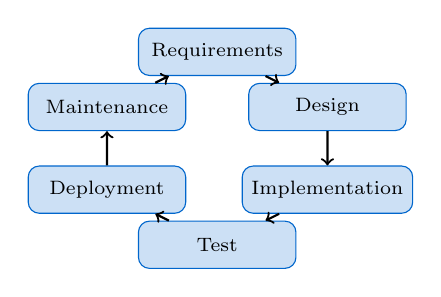
\begin{tikzpicture}[scale=0.7,
                phase/.style={rectangle, draw=primaryblue, fill=primaryblue!20, rounded corners, minimum width=2cm, minimum height=0.6cm, font=\scriptsize}
            ]
                \node[phase] (req) at (0, 2.5) {Requirements};
                \node[phase] (des) at (2, 1.5) {Design};
                \node[phase] (imp) at (2, 0) {Implementation};
                \node[phase] (test) at (0, -1) {Test};
                \node[phase] (dep) at (-2, 0) {Deployment};
                \node[phase] (maint) at (-2, 1.5) {Maintenance};

                \draw[->, thick] (req) -- (des);
                \draw[->, thick] (des) -- (imp);
                \draw[->, thick] (imp) -- (test);
                \draw[->, thick] (test) -- (dep);
                \draw[->, thick] (dep) -- (maint);
                \draw[->, thick] (maint) -- (req);
            \end{tikzpicture}
            \end{center}
        \end{column}
    \end{columns}
\end{frame}

%============================================================
\begin{frame}{Waterfall vs Agile}
    \begin{columns}
        \begin{column}{0.5\textwidth}
            \textbf{Waterfall Model}
            \begin{itemize}
                \item Sequential phases
                \item All requirements upfront
                \item No changes mid-project
                \item \textcolor{dangerred}{Problematic!}
            \end{itemize}
        \end{column}
        \begin{column}{0.5\textwidth}
            \textbf{Agile Model}
            \begin{itemize}
                \item Iterative approach
                \item 1--2 week sprints
                \item Continuous feedback
                \item \textcolor{successgreen}{Flexible!}
            \end{itemize}
        \end{column}
    \end{columns}
\end{frame}

%============================================================
\section{Scrum Framework}
%============================================================

\begin{frame}{Scrum Framework}
    \begin{block}{Most Popular Agile Framework}
        87\% of teams use Scrum (2022 State of Agile Report)
    \end{block}

    \vspace{0.3cm}

    \textbf{Scrum defines:}
    \begin{itemize}
        \item \textbf{Roles:} Scrum Master, Product Owner, Developers
        \item \textbf{Events:} Sprint, Sprint Planning, Daily Scrum, Review, Retrospective
        \item \textbf{Artifacts:} Product Backlog, Sprint Backlog, Increment
    \end{itemize}
\end{frame}

%============================================================
\section{Requirements}
%============================================================

\begin{frame}{Types of Requirements}
    \begin{columns}
        \begin{column}{0.5\textwidth}
            \begin{block}{Functional Requirements}
                User-visible features
                \begin{itemize}
                    \item ``User should register''
                    \item ``User should see posts''
                \end{itemize}
            \end{block}
        \end{column}
        \begin{column}{0.5\textwidth}
            \begin{block}{Non-Functional Requirements}
                Quality constraints (invisible)
                \begin{itemize}
                    \item ``Passwords as Bcrypt''
                    \item ``Load time < 1 second''
                \end{itemize}
            \end{block}
        \end{column}
    \end{columns}
\end{frame}

%============================================================
\section{User Stories}
%============================================================

\begin{frame}{User Story Format}
    \begin{center}
        \Large
        ``As a \textbf{[user persona]},\\
        I want \textbf{[action]}\\
        so that \textbf{[goal]}.''
    \end{center}

    \vspace{0.5cm}

    \begin{exampleblock}{Examples}
        \begin{itemize}
            \item ``As a \textbf{content creator}, I want to \textbf{create blogs} so I can \textbf{write posts for readers}.''
            \item ``As a \textbf{blog reader}, I want to \textbf{browse posts} so I can \textbf{find interesting content}.''
        \end{itemize}
    \end{exampleblock}
\end{frame}

%============================================================
\begin{frame}{INVEST Criteria}
    \begin{center}
    \begin{tabular}{cl}
        \toprule
        \textbf{I} & \textbf{Independent} -- Can be developed alone \\
        \textbf{N} & \textbf{Negotiable} -- Open to discussion \\
        \textbf{V} & \textbf{Valuable} -- Provides user benefit \\
        \textbf{E} & \textbf{Estimable} -- Team can estimate effort \\
        \textbf{S} & \textbf{Small} -- Fits in one sprint \\
        \textbf{T} & \textbf{Testable} -- Can verify completion \\
        \bottomrule
    \end{tabular}
    \end{center}
\end{frame}

%============================================================
\begin{frame}{Common User Story Problems}
    \begin{alertblock}{Too Large (violates ``Small'')}
        ``As content creator, I want to register with username, password, profile picture, and description''
    \end{alertblock}

    \begin{exampleblock}{Better -- Split into multiple stories}
        \begin{itemize}
            \item Register with username/password
            \item Add profile picture
            \item Add profile description
        \end{itemize}
    \end{exampleblock}
\end{frame}

%============================================================
\begin{frame}{Common User Story Problems (cont.)}
    \begin{alertblock}{Written from Developer Perspective}
        ``As developer, I want to add database index to optimize loading''
    \end{alertblock}

    \begin{exampleblock}{Better -- User-focused}
        ``As blog reader, I want blog posts to load quickly''
    \end{exampleblock}
\end{frame}

%============================================================
\section{Summary}
%============================================================

\begin{frame}{Key Takeaways}
    \begin{enumerate}
        \item Software projects need \textbf{identified need} + \textbf{funding}
        \item \textbf{Agile} welcomes change; \textbf{Waterfall} resists it
        \item \textbf{Scrum} is the most popular agile framework
        \item Requirements are \textbf{Functional} or \textbf{Non-Functional}
        \item User stories follow: ``As a..., I want..., so that...''
        \item Good user stories follow \textbf{INVEST} criteria
    \end{enumerate}
\end{frame}

%============================================================
\begin{frame}{Questions?}
    \begin{center}
        \Huge Questions?
    \end{center}
\end{frame}

\end{document}
